Release flow is a set of steps to perform to release upcoming version of software product.
Main aim of this document is to present simple and working model of software release
using semantic versioning~\cite{SemanticVersioning}, azure pipelines,
and mainline development~\cite{MainlineDevelopment}.
Mainline development is also known as GitHub flow.
Current document is motivated by Microsoft's ''Adopt a Git branching strategy'', see~\cite{AdoptGitStrategy}.
Below picture shows main idea of GitHub flow itself
\begin{figure}[H]
    \centering
    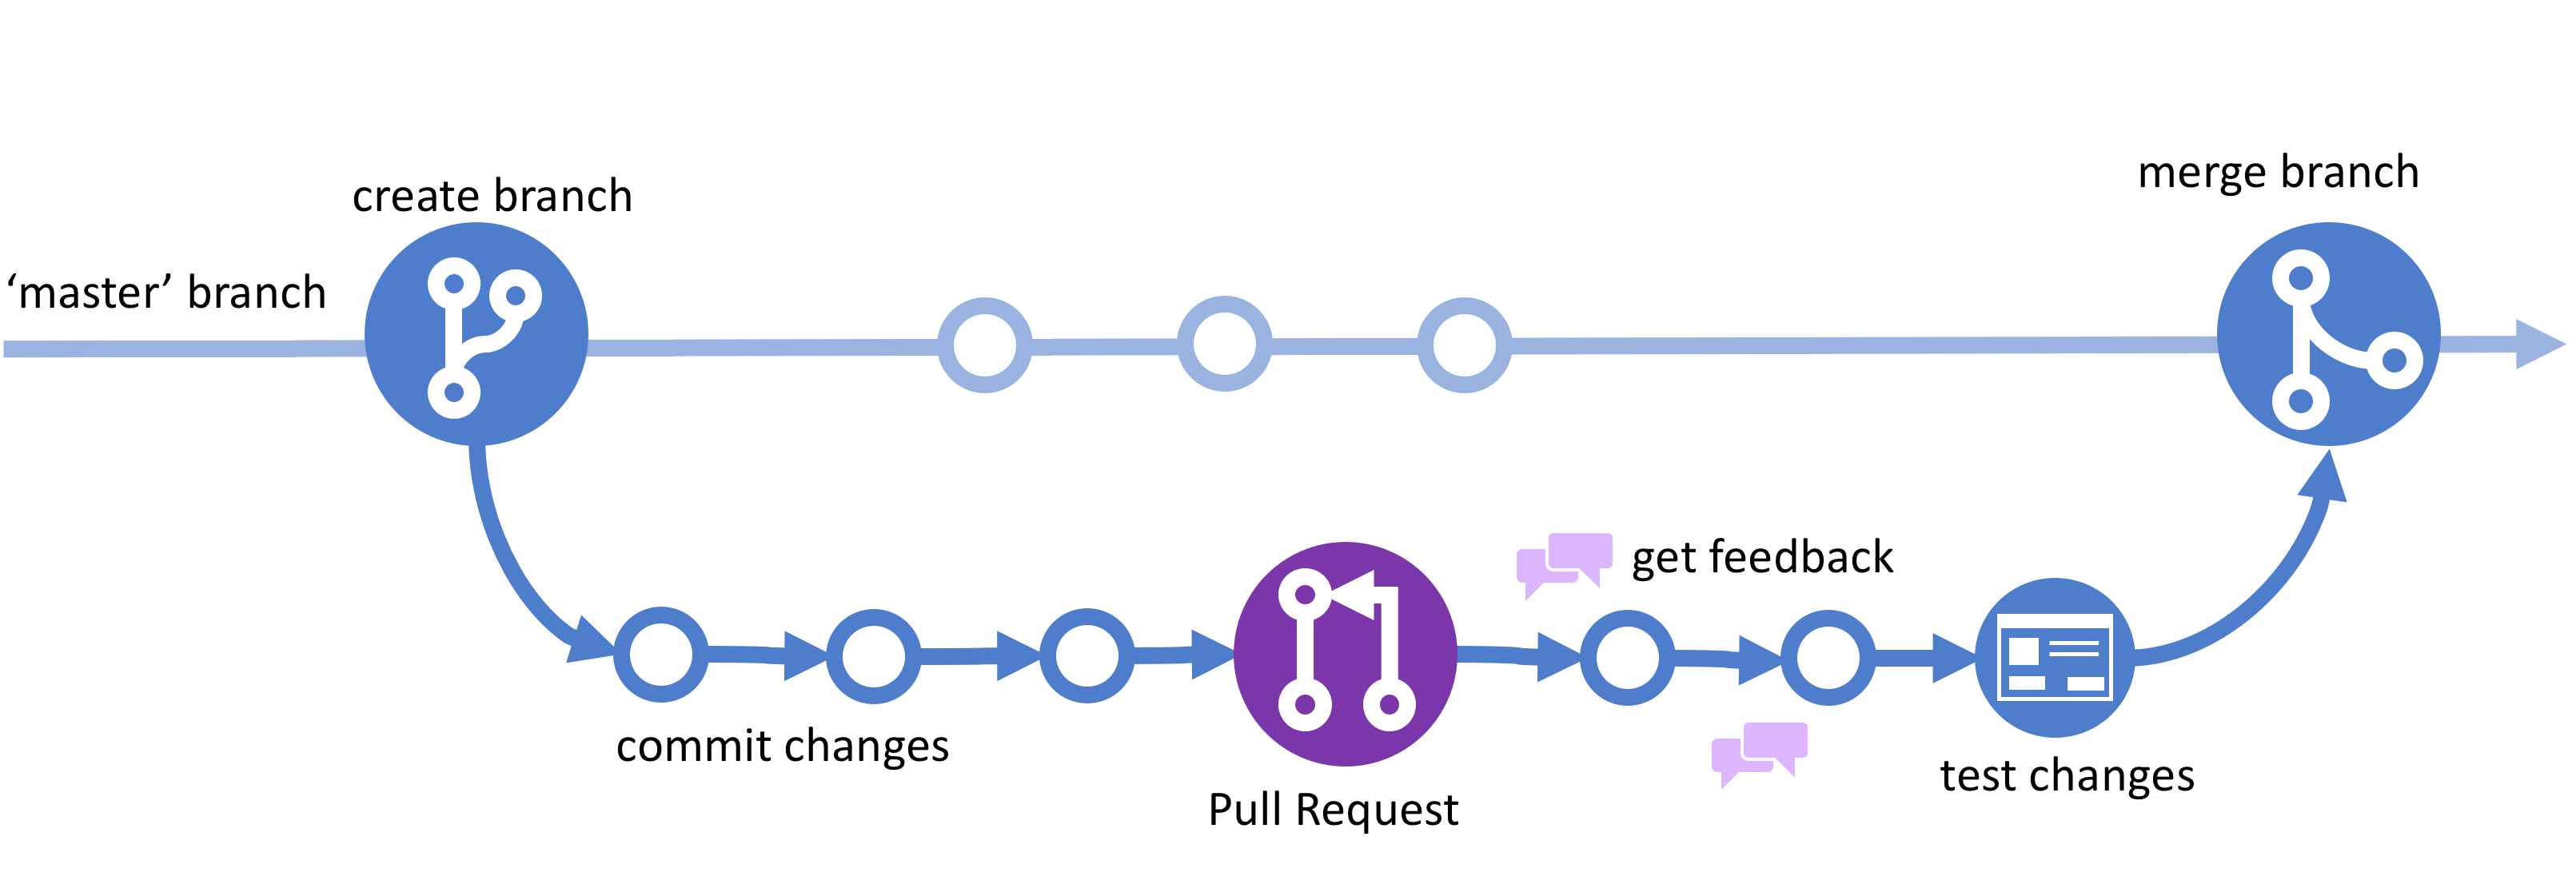
\includegraphics[width=1\textwidth]{../img/GitHub_Flow}
    ~\caption{GitHub Flow diagram.}
\end{figure}
\begin{itemize}
    \item \textbf{Master} -- branch that contains tested, validated and verified code, ready to be released.
    \item \textbf{Feature} -- branch that contains implementation of new feature according to sprint plan.
    Feature is branched from the \texttt{master} HEAD\@.
    \item \textbf{Bugfix} -- branch that contains non-critical bug fix.
    Bugfix is branched from the \texttt{master} HEAD\@.
    \item \textbf{Release/v*} -- branch that contains upcoming release state of software product.
    Release engineer decides what commit to be base of release branch.
    \texttt{Release/v*} is branched from the \texttt{master}.
    \texttt{Release/v*} is considered to be long-living branch, it should not be deleted after code is deployed.
    \texttt{Release/v*} branch is used to support current release of software product, after new release occurs
    team decides whereas to keep or to delete old release branch.
    After release complete \texttt{master} branch cherry-picks~\cite{CherryPick} from it.
    \item \textbf{Hotfix} -- branch that contains critical bug fix.
    It is used to patch production environment and must be released as quick as possible.
%    \item \textbf{Hotfix} -- branch is created from the latest deployed unit where error occurs,
%    for example \texttt{release/v*} branch.
%    Hotfixes are not stick to releases, they may be necessary in any deployed unit like DEV, QA environments,
%    depends on where error occurs.
%    This branch contains hotfix that should be deployed as soon as possible.
%    In case of hotfix branch, release to be done directly from it.
%    It means that after hotfix is finished new tag with patch increment to be created and pushed,
%    triggering CI/CD and deployment of hotfix to production.
\end{itemize}

\subsection{Release process}
Having all above, assume we have initial semantic version on our \texttt{master} branch as \texttt{v0.1.1},
and we must release upcoming version, our steps to perform are:
\begin{enumerate}
    \item Software engineer creates pull request from recent \texttt{feature} branch to \texttt{master} branch,
    this pull request triggers Continuous Integration (CI) to start, CI runs tests, code quality checks etc.,
    but deployment won't be started yet, only CI\@.
    \item After all CI checks passed, pull request reviewed by team and every comment from code review is fixed --
    it is ready to be merged from \texttt{feature} branch to \texttt{master} branch.
    No CI/CD pipeline triggered by the merge.
    \item Next, release engineer reviews software product changes using \texttt{CHANGELOG} or \texttt{git compare}.
    Release engineer makes decision which part of semantic version to increment.
    For example, release engineer decided that minor version should be incremented then our version becomes,
    for example \texttt{v0.1.1 -> v0.2.0}
    \item Release engineer creates new release as follows
    \begin{itemize}
        \item Checkout to release branch: \texttt{git checkout -b release/v0.2.0}
        \item Work on release committing some minor fixes
        \item Push release branch to remote: \texttt{git push origin release/v0.2.0}
        \item Create tag: \texttt{git tag -a v0.2.0 -m "Release v0.2.0"}
        \item Push tag: \texttt{git push origin v0.2.0}
    \end{itemize}
    \item After new tag is pushed the CI/CD pipeline is triggered by that event~\cite{AzurePipelinesTriggers}.
    There are three deployments scheduled: DEV, QA, UAT\@.
    Environments QA and UAT are to be approved by designated personnel before deployment starts,
    DEV to be deployed without manual approve.
    \item Finally, \texttt{master} branch cherry-picks~\cite{CherryPick} from \texttt{release/v0.2.0} after deployment is complete.
\end{enumerate}
Entire release process is shown on the picture below
\begin{figure}[H]
    \centering
    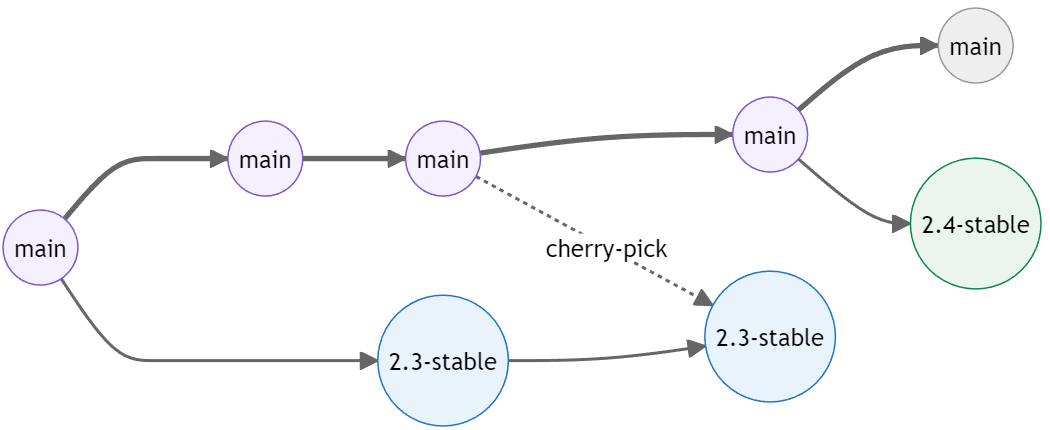
\includegraphics[width=1\textwidth]{../img/GitLab_Flow}
    ~\caption{GitLab Flow diagram~\cite{GitLabFlow}.}
\end{figure}

\subsection{Hotfix strategy}